\begin{mainquestion}{ledloadline}{LED Load-Line}

The red LED we investigated in Lab 2 (model 307E) has the following I-V curve shown below. You may assume a temperature of 25~°C for this problem.

\begin{center}
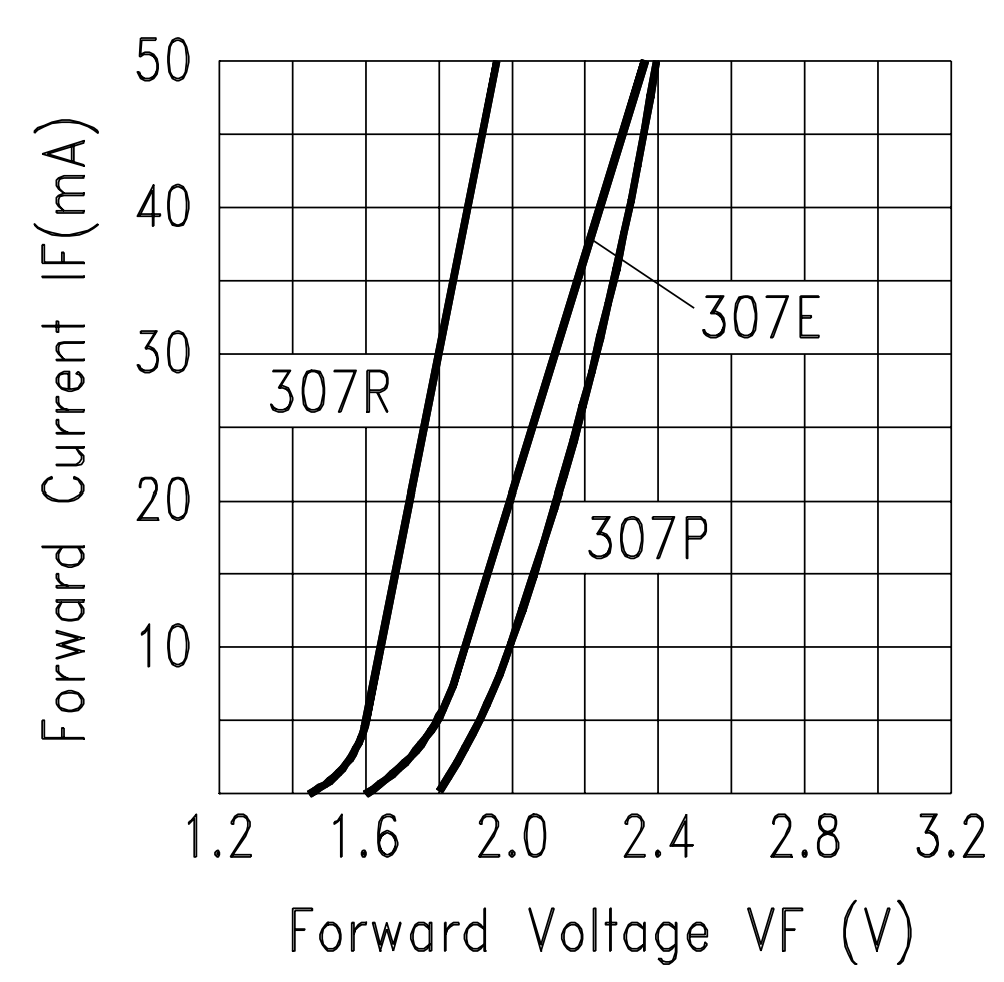
\includegraphics[width=4in]{questionbank/diodes/led_iv_curve/v0/iv_curve.png}
\end{center}

% =========================================================
\begin{partquestion}{basicloadline}
{Consider placing this LED in series with a fresh CR-2032 battery and a 1~k$\Omega$ resistor. Use load-line analysis to determine the voltage across the diode and the current through the diode.}

\begin{answer}
A new CR-2032 battery will provide $V_{\text{batt}} = 3\text{ V}$ of potential. The load-line equation for the circuit with a battery and 1~k$\Omega$ resistor is found from Ohm's law:

\[
I_D = \frac{V_{\text{batt}} - V_D}{R} = (3 - V_D)\text{ mA}
\]

(Note the units are in mA since the resistor was in k$\Omega$.) We can plot this line on the graph in red. The graph's $y$-intercept (note this is not at $V_D = 0$, rather at $V_D = 1.2$) is 1.8 mA, and the $x$-intercept is 3~V (when $I_D = 0$).

\begin{center}
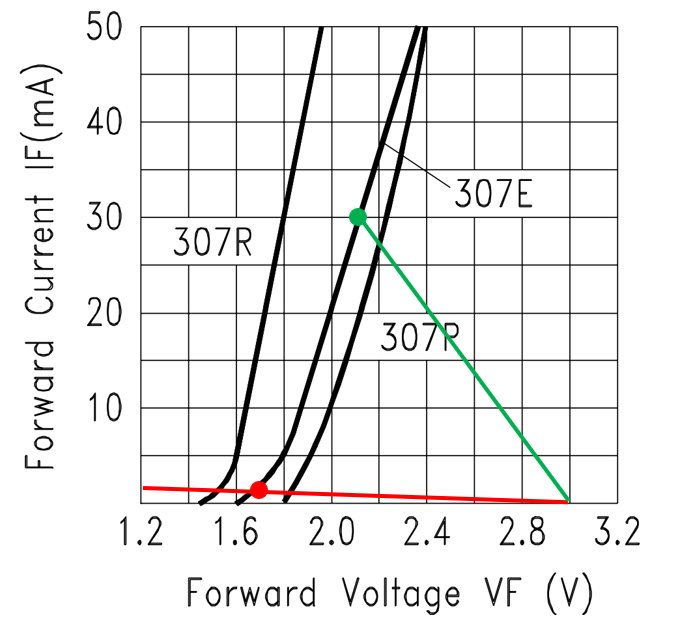
\includegraphics[width=4in]{questionbank/diodes/led_iv_curve/v0/iv_curve_traced.png}
\captionof*{figure}{Load-line construction for the LED circuit for part (\cref{prob:ledloadline:basicloadline}) (shown in red), and part (\cref{prob:ledloadline:resistorselection}) (shown in green)}
\end{center}

This intersects the 307E curve at approximately:
\begin{itemize}
  \item Forward voltage: $V_D \approx 1.7\text{ V}$
  \item Forward current: $I_D \approx 1.3\text{ mA}$
\end{itemize}
\end{answer}
\end{partquestion}

% =========================================================
\begin{partquestion}{ledbrightness}
{With the 1~k$\Omega$ resistor, you may be disappointed by the  brightness. Explain why that is.}

\begin{answer}
We are barely operating above the forward voltage cutoff level. The resulting low current (1.3 mA) is not a lot of current for typical LEDs such as this one, which are typically used in situations where there is an order of magnitude more current, providing a much brighter LED.
\end{answer}
\end{partquestion}

% =========================================================
\begin{partquestion}{resistorselection}
{After reviewing the salient details in the \href{https://www.jameco.com/Jameco/Products/ProdDS/697522.pdf}{data sheet}, again use load-line analysis to calculate a suitable resistor value that will continuously provide as bright an LED as possible while staying within the specified absolute maximum ratings. Make sure you choose a realizable resistor value (assume \href{https://asenergi.com/pdf/resistors/standard-resistor-values-e24.pdf}{E24 series}---also in Hambley Table B.1).}

\begin{answer}
According to the data sheet, the 307E LED is a Red Diffused LED with a High Efficiency Red source. The maximum rating at 25~°C for continuous forward current is given as 30 mA. From the I-V curve of the LED, this requires a LED forward voltage of about 2.1~V. Using load-line analysis, we can draw a line between this point and the $x$-intercept (which remains at 3~V since the battery is unchanged) in green. The slope is:

\[
\frac{0\text{ mA} - 30\text{ mA}}{3\text{ V} - 2.1\text{ V}} = -33.3\text{ mS}
\]

The slope equals the negative reciprocal of the resistance:

\[
R = \frac{1}{33.3\text{ mS}} = 30\text{ }\Omega
\]

This represents a lower bound on $R$---any lower value would create a current higher than the maximum allowed forward current of 30 mA. Fortunately, the E24 series contains a 30 $\Omega$ resistor, so we can use that! \it{N.B.}: This is the theoretical minimum resistance under the simplified assumptions. A practical design would generally include margin rather than operate continuously at the absolute maximum rating.
\end{answer}
\end{partquestion}

% =========================================================
\begin{partquestion}{ambienthot}
{Repeat part (\cref{prob:ledloadline:resistorselection}) assuming the LED is operating at an ambient temperature of \qty{75}{\celsius} (see \href{https://www.jameco.com/Jameco/Products/ProdDS/697522.pdf}{datasheet})}

\begin{answer}
On the \textbf{Absolute Maximum Ratings} table, the datasheet provides a linear derating factor for the maximum continuous current of \qty{0.4}{\milli\ampere\per\celsius} above \qty{50}{\celsius}. We can calculate our new maximum current using this derating factor:
\[I_{\text{max,75C}} = 30 - 0.4(75 - 50) = \qty{20}{\milli\ampere}\]
Alternatively, Figure 4 also provides the same information via the slope of the 307E curve on the following graph:

\begin{center}
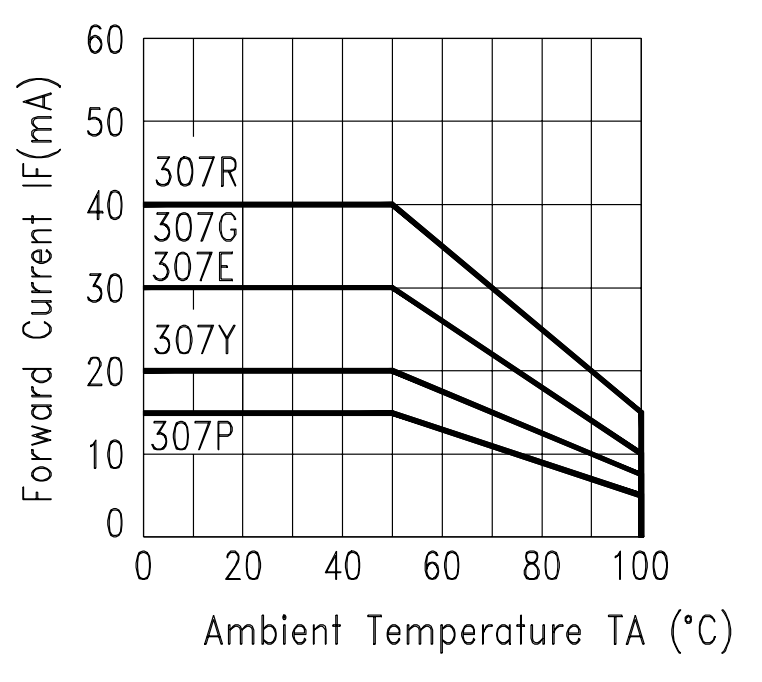
\includegraphics[width=4in]{questionbank/diodes/led_iv_curve/v1/fig4.png}
\end{center}

Now we can just repeat the previous load line analysis for this new target.

\begin{center}
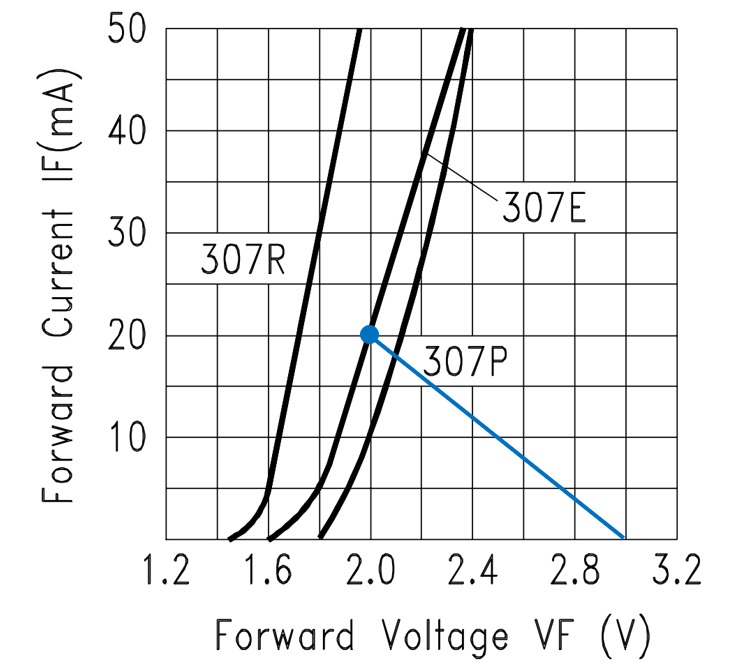
\includegraphics[width=4in]{questionbank/diodes/led_iv_curve/v1/load_curve_hot.png}
\end{center}

\[
\frac{0\text{ mA} - 20\text{ mA}}{3\text{ V} - 2.0\text{ V}} = -20\text{ mS} \rightarrow 50\text{ }\Omega
\]
The closest value in the E24 series with no less than \qty{50}{\ohm} of resistance is \qty{51}{\ohm}.
\[R_{\text{75C}} = \qty{51}{\ohm}\]

\end{answer}
\end{partquestion}

\end{mainquestion}
